
It has been widely documented that the use of the $Q_1 \times P_0$ element is not without problems. Aside from the 
consequences it has on the FE matrix properties, we will here focus on another unavoidable side effect: 
the spurious pressure checkerboard modes. 
\index{general}{Pressure Smoothing} 
\index{general}{Checkerboard mode}

These modes have been thoroughly analysed \cite{grsi94,chpc95,sagl81a,sagl81b}.
They can be filtered out \cite{chpc95} or simply smoothed \cite{legs79}.

On the following figure (a,b), pressure fields for the lid driven cavity experiment 
are presented for both an even and un-even number of elements. We see that 
the amplitude of the modes can sometimes be so large that the 'real' pressure is 
not visible and that something as simple as the number of elements in the 
domain can trigger those or not at all.

\begin{center}
a)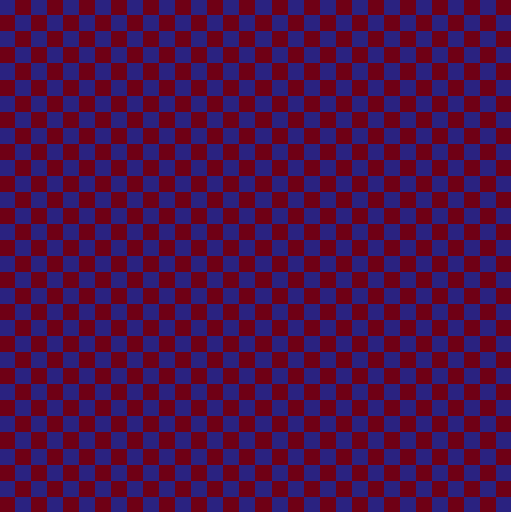
\includegraphics[width=3cm]{images/checkerboard/p_el}
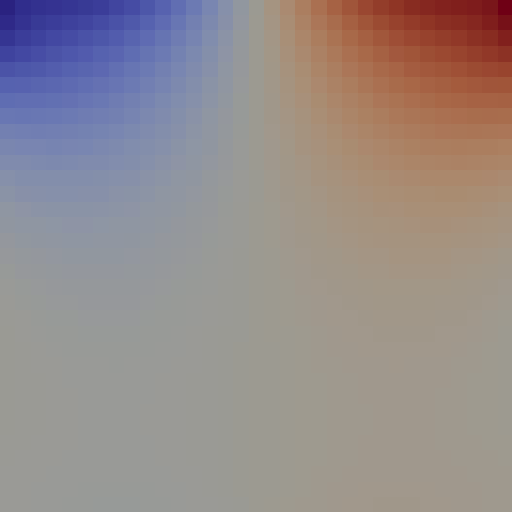
\includegraphics[width=3cm]{images/checkerboard/p_el_33x33}
b)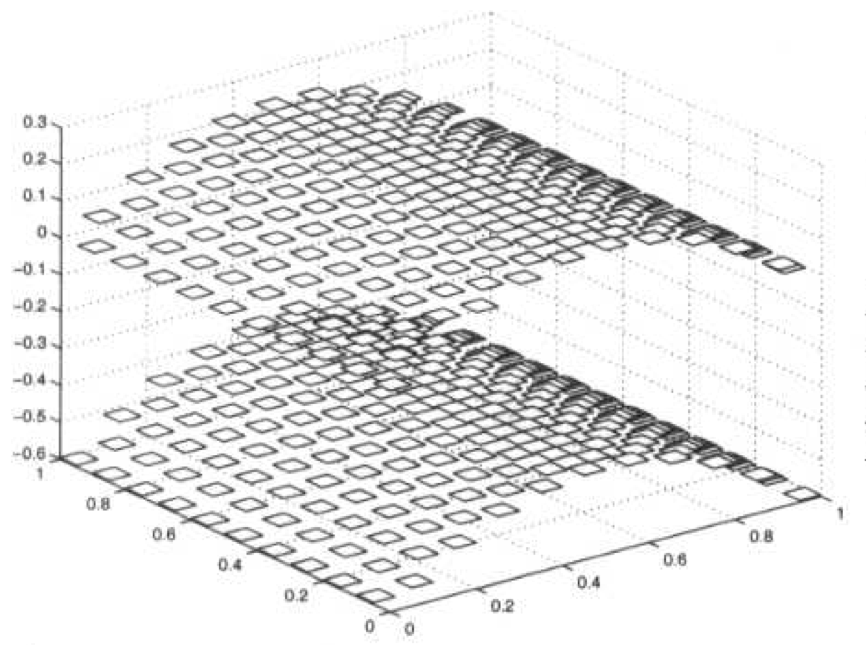
\includegraphics[width=5cm]{images/checkerboard/press_doneahuerta}
c)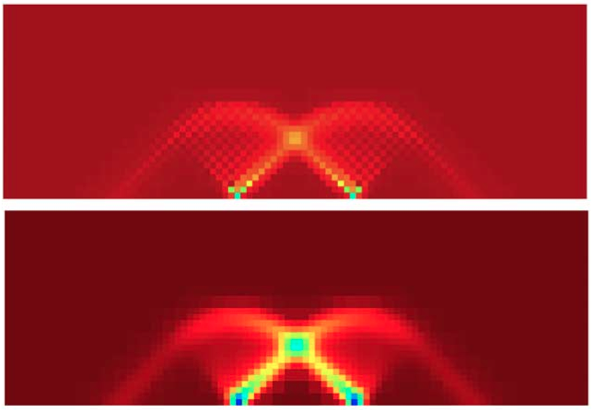
\includegraphics[width=5cm]{images/checkerboard/douarpunch}\\
{\captionfont a) element pressure for a 32x32 grid and for a 33x33 grid;\\ 
b) image from \cite[p307]{dohu03} for a manufactured solution;\\ 
c) elemental pressure and smoothed pressure for the punch experiment \cite{thfb08}}
\end{center}

The easiest post-processing step that can be used (especially when a regular grid is used) 
is explained in \cite{thfb08}: "The element-to-node interpolation is performed by
averaging the elemental values from elements common to each node; 
the node-to-element interpolation is performed
by averaging the nodal values element-by-element. This
method is not only very efficient but produces a smoothing
of the pressure that is adapted to the local density of the
octree. Note that these two steps can be repeated until a
satisfying level of smoothness (and diffusion) of the pressure field is attained."

In the codes which rely on the $Q_1 \times P_0$ element, the (elemental) pressure
is simply defined as 
\begin{lstlisting}
p=np.zeros(nel,dtype=np.float64)  
\end{lstlisting}
while the nodal pressure is then defined as 
\begin{lstlisting}
q=np.zeros(nnp,dtype=np.float64)  
\end{lstlisting}
The element-to-node algorithm is then simply (in 2D):

\begin{lstlisting}
count=np.zeros(nnp,dtype=np.int16)  
for iel in range(0,nel):
    q[icon[0,iel]]+=p[iel]
    q[icon[1,iel]]+=p[iel]
    q[icon[2,iel]]+=p[iel]
    q[icon[3,iel]]+=p[iel]
    count[icon[0,iel]]+=1
    count[icon[1,iel]]+=1
    count[icon[2,iel]]+=1
    count[icon[3,iel]]+=1
q=q/count
\end{lstlisting}

Pressure smoothing is further discussed in \cite{hulb79}.

\improvement[inline]{produce figure to explain this}

\improvement[inline]{link to proto paper }

\improvement[inline]{link to least square and nodal derivatives}






